\newpage\section{Desenvolvimento}

Este capítulo discute o funcionamento dos algoritmos desenvolvidos para a coordenação da \rssf em conjunto com 
\vants. As próximas seções descrevem o problema tratado e apresentam soluções para a resolução destes problemas.


\subsection{Descrição do Problema}

Este trabalho preocupa-se em pesquisar e desenvolver estratégias para a
coordenação de uma rede de sensores heterogênea. A rede em questão deve ser
utilizada para prover tarefas de monitoramento e vigilância de um ambiente de
interesse. Como ferramentas para se realizar estas tarefas de monitoramento são
utilizados nós sensores terrestres equipados com diversas interfaces de
sensoriamento e \vants também equipados com interfaces de sensoriamento e
enlaces de comunicação sem fio.

A justificativa e motivação para a utilização destes diferentes tipos de nós
sensores encontra-se no fato de que um nó sensor terrestre usual apresenta
capacidade computacional reduzida. Portanto, estes tipos de nós são incapazes de
cumprir todas as tarefas da rede individualmente. Em contrapartida, estes nós
sensores convencionais geralmente possuem custos reduzidos, o que propicia o uso
de vários sensores para a realização de missões. 

\uavs podem variar em tamanhos, formas, configurações e propósitos, adequando-se
a diversos cenários de aplicação. Neste trabalho, justifica-se o uso de
\emph{Mini-UAVs} (UAVs Multi-Missão), que são aeronaves de custo não tão elevado
quando comparados aos custos de aeronaves de grande porte. Portanto, uma
alternativa interessante é a utilização de \emph{Mini-UAVs} carregando uma
variedade de sensores específicos (sensores como câmeras de alta resolução,
infra-vermelho, GPS, etc) e que possuam poder computacional superior aos nós
sensores terrestres, permitindo assim que os \vants possam realizar missões e
medidas mais sensíveis e específicas.

Esta relação entre sensores terrestres simples e de baixo custo e \vants
relativamente mais caros justifica o uso de vários sensores simples espalhados
pela área de interesse em conjunto com alguns poucos, ou apenas um, \vant para
realizar as tarefas mais específicas. 

Por fim, o problema tratado é o desenvolvimento de estratégias eficientes para detecção de um evento através dos
nós sensores mais simples e garantir que as mensagens sejam entregues aos \vants
mais hábeis a tratar o evento de forma específica.

Dentre uma infinidade de exemplos de monitoramento de áreas de interesse,
podem ser citados:

\begin{description}
 \item [Áreas Militares de Acesso Restrito:] Locais de acesso proibido, onde se deseja detectar a presença de intrusos.
 \item [Detecção de Fenômenos Físicos:] São áreas onde se pretende detecctar a ocorrência de fenômenos como alteração de
temperatura, umidade, sons, etc.
 \item [Observação de Animais:] Aplicações em que o objetivo seja o monitoramento de espécies de animais, como, por exemplo,
a presença de uma espécie incomum em uma determinada área.
\end{description}



Observados os problemas e exemplos expostos anteriormente, este trabalho apresenta algumas soluções para se aprimorar
a utilização de veículos aéreos não tripulados em conjunto com redes de sensores sem fio.

Resumidamente, os algoritmos desenvolvidos são:

\begin{description}

	\item[ (a) Distribuição de Ferormônio: ] o \vant sobrevoa continuamente
a área de interesse da aplicação. Enquanto sobrevoa esta área, o \vant deve se
comunicar com os nós sensores que se encontram abaixo do mesmo, estes nós
armazenam um valor com a intensidade do sinal com que a mensagem foi recebida.
Neste momento é formado um gradiente que corresponde a um rastro artificial da aeronave.

	\item[ (b) Detecção e Propagação do Evento:] quando um evento é
detectado, os nós sensores terrestres devem realizar uma negociação a fim de
enviar uma mensagem de alarme para os \vants presentes na área. Esta mensagem
deve encontrar o rastro de ferormônio formado em (a) e prosseguir até o \vant
mais hábil para tratar o evento ocorrido.

	\item[ (c) Reforço de Conectividade da Rede:] algoritmo utilizado para reforçar a conectividade da rede em casos de falhas em algum nó.

%% Este aqui vai par os trabalhos futuros

% 	\item[ (c) \emph{Tracking} e Perseguição do Intruso: ] no momento em que
% os nós sensores detectam a presença de um dado evento, como exemplo o caso de um
% intruso, providências devem ser tomadas para que o mesmo alarme de evento não
% seja repetido. Por exemplo, o nó sensor X percebe a presença de um intruso na
% área, poucos segundos depois o nó Y também percebe o mesmo intruso, se ambos os
% nós enviarem um alarme aos \vants pode ocorrer carga excessiva na rede, bem como
% gerar confusão entre os \vants, pois os mesmos são interrompidos e reprogramados
% a cada alarme recebido. Portanto, na ocorrência de um evento, os nós da micro
% região onde onde houve a detecção devem alterar seu modo de trabalho, realizando
% assim uma perseguição e rastreamento, marcando uma trilha de mobilidade do
% evento, ao invés de soar os alarmes novamente.

%\item[ (b) Reforço dos Rastros de Ferormônio:] Em situações em que se utiliza mais de uma aeronave pode se 
%tornar interessante desenvolver uma política de reforço dos rastros de ferormônio construídos em (a) por cada \vant.
%Nesse caso, cada \vant pode reforçar o gradiente de todos os outros, desde que seus rastros se encontrem em algum ponto
%da área de interesse.

\end{description}

As próximas seções discutem o problema apresentado em diferentes perspectivas, apresentando suas peculiaridades e possíveis
soluções. Os algoritmos são introduzidos em uma sequência lógica para que se torne possível o entendimento do problema em questão. Vale 
ressaltar que esta ordem foi escolhida para um melhor entendimento do problema, visto que cada seção apresenta dependência em relação aos conceitos
apresentados nas seções anteriores. 

\subsection{Detecção de Eventos}
Para que um sistema de monitoramento realize seu papel de forma eficaz, espera-se, no mínimo, que este seja capaz de detectar eventos. Todo o funcionamento
de um sistema deste tipo depende da detecção dos eventos de interesse. Contudo, o foco deste trabalho não está no desenvolvimento de algoritmos para 
detecção de eventos. Portanto, adotou-se uma abordagem básica para a detecção de eventos pela \rssf, visto que a preocupação principal deste trabalho não se concentra neste problema.

A estratégia de detecção dos eventos de interesse escolhida pode ser considerada simples. Entretanto, apresenta-se eficaz para o desenvolvimento deste trabalho.
Cada nó sensor dá rede possui sensores dos mais variados tipos: umidade, temperatura, pressão, eletro-magnético, etc. Cada um destes sensores pode ser
configurado de modo que possua um limite\footnote{O termo limite pode ser encontrado em literaturas internacionais como \emph{threshold}} aceitável de medição em determinado parâmetro. Definidos os limites, são agendadas algumas medições para aquele sensor. Em caso de uma medição exceder o limite aceitável
para aquele parâmetro o nó sensor pode considerar este fenômeno como um evento de interesse detectado. Se a medição não exceder o limite, o nó simplesmente
deverá agendar outra leitura em tempo futuro.

O algoritmo a seguir demonstra o algoritmo em formato simplificado. \\

\begin{algorithm}[H]
	\SetAlgoLined
	
	\SetKwFunction{realizarMedicaoNoAmbiente}{realizarMedicaoNoAmbiente}
	\SetKwFunction{acionarAlarme}{acionarAlarme}
	\SetKwFunction{agendarAproximaMedicao}{agendarAproximaMedicao}

	\Entrada{Parâmetros do Ambiente}
	
	\Enqto{ainda existem medições agendadas}{
		medicao = \realizarMedicaoNoAmbiente() \;
		\Se{medicao maior que LIMITE}{
			\acionarAlarme()\;
		}
			\agendarAproximaMedicao(AtrasoParaProximaMedicao) \;
	}
\caption{Algorítmo para a detecção de eventos no ambiente.}
\end{algorithm}


\subsection{Distribuição de Feromônio}
Este algoritmo tem como objetivo a construção de um rastro de feromônios sobre a rede de sensores. A construção deste rastro possibilita que cada \vant receba mensagens de
maneira mais rápida e mais eficiente, bem como otimiza os caminhos para que uma mensagem alcance seu destino.

 \begin{figure}
 \centering
 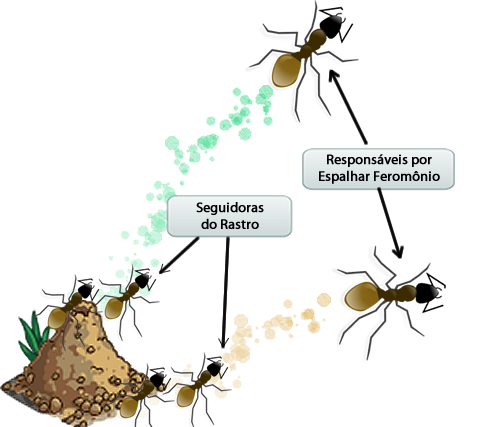
\includegraphics[width=12cm]{pictures/ants.png}
 \caption{Fenômeno Biológico de Distribuição de Feromônio.}
  \label{fig:ants}
 \end{figure}

Para a composição destes rastros é utilizada uma heurística inspirada em fenômenos biológicos, mais especificamete no comportamento de formigas quando buscam alimento.
O princípio deste comportamento, de forma simplificada,  é que uma formiga libera seu rastro através de um caminho no momento em que começa sua viagem em busca de alimento. Este rastro é composto por feromônios que exalam um odor específico para marcar o caminho percorrido. Um ponto importante a se ressaltar é que este rastro se evapora com o passar do tempo, isto, por fim, resulta em um gradiente que decresce de acordo com o tempo. Consequentemente, este caminho possuirá duas extremidades, uma extremidade com baixo valor de feromônio (início do caminho) e uma extremidade com altíssima concentração de feromônio (posição atual da formiga). Este rastro possibilita que a formiga (detentora do rastro) possa ser alcançada por qualquer outro indivíduo (outras formigas) que possua capacidades de interpretar o odor do feromônio.

A figura \ref{fig:ants} demonstra o fenômeno descrito.



Inspirado no comportamento anteriormente descrito, torna-se possível criar uma adaptação do mesmo para implementação no uso de redes de sensores sem fio em conjunto com veículos aéreos não tripulados. Para isso, basta que se considere um \vant como uma formiga capaz de produzir um rastro feromônio. Este rastro resultará em uma espécie de \emph{backbone} de feromônios que otimizará a entrega de mensagens destinadas ao \vant. A estratégia utilizada para que este comportamento fosse mapeado para uma rede de sensores pode ser dividida em duas responsabilidades:

\subsection{Entrega de Feromônios pelos \vants}
Cada \vant sobrevoando a área de interesse exala seus feromônios digitais periodicamente durante seu vôo. Utilizando recursos de comunicação sem fio, o \vant simplemeste mente enviará pacotes \emph{beacon} periodicamente em \emph{broadcast}. Este comportamente garante que os pacotes são enviados a todo momento para todos os nós sensores que se encontram no alcance do raio de comunicação do \vant. Um ponto interessante a se ressaltar é o \vant deve enviar, em cada pacote, um atributo que indique o "sabor" de feromônio que este \vant possui. Isto garante que no caso de vários \vants sobrevoando a área de interesse os rastros não se sobreponham, de modo que em um mesmo local possam ser armazenador rastros distintos.

A figura \ref{fig:broadcast} demonstra o item apresentado.

 \begin{figure}[h!]
 \centering
 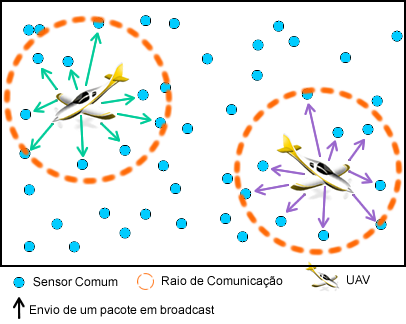
\includegraphics[width=10cm]{pictures/broadcast.png}
 \caption{Envio de um pacote em broadcast. Cada cor nas setas representa um sabor de feromônio.}
  \label{fig:broadcast}
 \end{figure}

\subsection{Armazenamento por parte dos Nós Sensores}
Os nós sensores espalhados pela área são responsáveis por armazenar os feromônios distribuídos pelos \vants, de modo a reproduzirem os rastros. Cada nó, ao receber um pacote enviado por um \vant deverá armazenar o sabor de feromônio recebido. Esta ação, quando observada em nível macro (todas as micro-ações produzidas por cada nó), resultará em um comportamento global, construindo rastros de feromônios digitais que representam os caminho percorridos por cada \vant dentro da área de interesse. 

 \begin{figure}[h!]
 \centering
 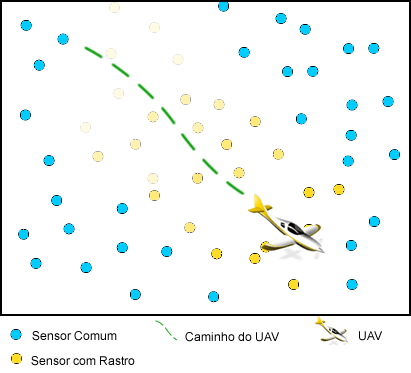
\includegraphics[width=10cm]{pictures/flat_pheromone.png}
 \caption{Pheromônios esmaecendo em função do tempo.}
  \label{fig:flat}
 \end{figure}

Além de armazenar o valor de feromônio recebido, o nó sensor deve agendar uma tarefa interna para reduzir seu valor de feromônio de acordo com o tempo. Um exemplo de tarefa é reduzir a cada 300 segundos o valor de feromônio armazenado a uma taxa de 10\%, de modo a simular a evaporação do feromônio. Esta evaporação garante que o rastro mantenha-se em maior concentração de feromônio na extremidade onde se encontra o \vant, e, em menor concentração na extremidade onde o rastro se originou.



Cada nó sensor armazenando os valores de feromônios representa o caminho por onde o \vant sobrevoou. Contudo, este rastro ainda pode conter certas ambiguidades. Observando-se o fato que diversos nós sensores recebem o mesmo valor de feromônio, verifica-se que em uma mesma região contida no raio de alcance do \vant (considerando-se que a propagação do sinal ocorre em formato circular) existem diversos nós sensores representando a mesma quantidade de feromônio, como demonstrado na figura \ref{fig:flat}. Ainda que os valores evaporem com o tempo, seguindo esta tendência, os nós sensores evaporarão com a mesma proporção, resultando em um rastro que somente encaminhará as mensagens a uma região (do mesmo tamanho do raio de propagação do \vant), não a um ponto específico na rede. Neste caso, encaminhar a mensagem a uma região pode não ser o ideal, visto que a mensagem não encontraria um sentido correto para ser encaminhada.



Para sobrepor esse problema, pode-se adicionar uma restrição ao se armazenar um valor de feromônio em um dado nó sensor. Neste caso, em específico, utiliza-se a informação de intensidade com que o pacote foi recebido (RSSI) pelo nó sensor. A informação recebida garante que se armazene valores de feromônio proporcionais à distância entre os nós sensores e o emissor dos pacotes. Este armazenamento promoverá, em nível macro, um rastro em formato de gradiente, que será resultante da variação dos valores de feromônio em relação ao tempo em que o nó sensor recebeu o pacote e à distância entre o nó sensor e o \vant emissor do pacote. Este gradiente é demonstrado na figura \ref{fig:gradient}.

 \begin{figure}[h!]
 \centering
 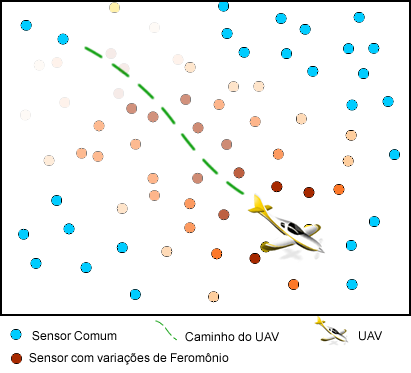
\includegraphics[width=10cm]{pictures/gradient.png}
 \caption{Pheromônios esmaecendo em função do tempo e da distância relativa ao \vant. Os toms de vermelho variam de acordo com a distância do nó sensor em relação ao \vant, bem como varia a transparência do nó em relação ao tempo.}
  \label{fig:gradient}
 \end{figure}


\subsection{Propagação de Eventos}
Uma vez detectado um evento de interesse, espera-se que o sistema seja capaz de reportá-lo ao \vant mais adequado para tratar o fenômeno com maior granularidade. Para o alcance de tal objetivo é utilizado um algoritmo de propagação de eventos. Este algoritmo integra os dois algoritmos anteriores, de modo que se torne possível a entrega dos eventos aos \vants.

O primeiro passo para o funcionamento deste algoritmo é a definição de alarme. Neste contexto um alarme é considerado como uma estrutura de dados responsável por carregar informações acerca do evento ocorrido. A estrutura de um alarme é formada por:

\begin{description}
	\item[\emph{Position}:]  Representa a posição em que o evento foi detectado.
	\item[\emph{TimeStamp}:] Informa o momento em que o alarme foi disparado.
	\item[\emph{PheromoneAmmount}:] Indica a quantidade atual de feromônio presente no alarme. Esta quantidade de feromônio é o principal atributo presente nesta estrutura de dados, pois será atualizada cada vez que o alarme for repassado.
	\item[\emph{Flavor}:] Fornece o "sabor" de feromônio mais propício a tratar este evento. Por exemplo, no caso da detecção de um evento sonoro, o sabor do alarme seria "\emph{noise}", de modo que este alarme somente deve ser repassado para nós sensores que possuam feromônios do sabor \emph{noise}.
\end{description}

O funcionamento básico desta propagação de eventos baseia-se em repassar o alarme do ponto inicial (ponto de detecção do evento) ao ponto final (posição do \vant). Visto que neste ponto já existem diversos gradientes formados pelos rastros dos \vants, a tarefa do nó sensor detector do evento resume-se em determinar o "sabor"  que mais se adequa ao evento em questão e encaminhar o alarme, de modo que o mesmo alcance seu destino (\vant mais apropriado).

Para a propagação do alarme criado, o nó sensor deve encaminhá-lo somento a outros nós sensores que estejam dentro do mesmo rastro de feromônio. Uma observação importante neste método é que o alarme só deve ser encaminhado para nós sensores que possuam concentração de feromônio superior ao do nó sensor criador do alarme. Para que essa premissa seja garantida,  torna-se imprescindível que a estrutura de Alarme carregue a informação da quantidade de feromônio presente no alarme. Seguindo-se esta idéia, o nó sensor detector deve encaminhar seu alarme em mensagens do tipo \emph{broadcast}, de modo que seus vizinhos recebem a informação de alarme. 

Uma vez que um vizinho do nó sensor propagador receber o pacote contendo o alarme, deverá analisar o alarme recebido e decidir se encaminha a mensagem ou não.  Se a quantidade de feromônio armazenada no nó sensor receptor for menor que a quantidade do alarme, o nó receptor simplesmente deve descartar o alarme. Contudo, se a quantidade armazenada no nó receptor for superior à quantidade de feromônio recebida, o nó receptor deve atualizar atualizar o valor de feromônio do alarme com seu próprio valor e repassar a mensagem também em formato de \emph{broadcast}. 

A execução das pequenas e locais ações anteriores acarretará em um comportamento global em toda a rede de sensores. Estas interações entre os nós sensores promoverão a entrega da mensagem contendo o alarme ao \vant que estiver sobrevoando a área de interesse no momento em que se detectou o evento.

O algoritmo básico, em psedocódigo, para este fenômeno pode ser visualizado abaixo: \\


\begin{algorithm}[H]
	\SetAlgoLined
	
	\SetKwFunction{minhaQuantidadeDeFeromonio}{minhaQuantidadeDeFeromonio}
	\SetKwFunction{encaminharAlarme}{encaminharAlarme}

	\Entrada{Objeto Alarme}

	\Se{ alarme.quantidadeDeFeromonio < \minhaQuantidadeDeFeromonio() }{
			alarme.quantidadeDeFeromonio = \minhaQuantidadeDeFeromonio()\;
			\encaminharAlarme(alarme);
		}
	
\caption{Algoritmo para a propagação de eventos.}
\end{algorithm}


Uma particularidade interessante deste algoritmo é que podem exister regiões na área de interesse em que ainda não se existe a presença de rastros de feromônio. Contudo, esta questão apresenta-se discutível, pois poderia-se considerar que o sistema só entraria em funcionamento no momento em que toda área já estivesse coberta pelo \vant. Entretanto, esta premissa não pode ser garantida em todos os casos. Para que este problema seja contornado, pode ser proposta uma variação deste algoritmo em que quando um nó sensor detectar um evento e o mesmo não possuir rastro de feromônio, este nó deverá encaminhar a mensagem para um de seus vizinhos, na esperança de que este visinho possua rastros. Existem algumas medidas para que se escolha o vizinho mais adequado para receber a mensagem de alarme. Contudo, devido a extensibilidade da explicação, não serão abordadas neste trabalho. Porém, vale ressaltar que esta particularidade ocorre em poucos casos e será abordada novamente no capítulo de resultados.

 A figura \ref{fig:app} demonstra um exemplo do funcionamento básico da propagação de eventos.
 

 \begin{figure}[h!]
 \centering
 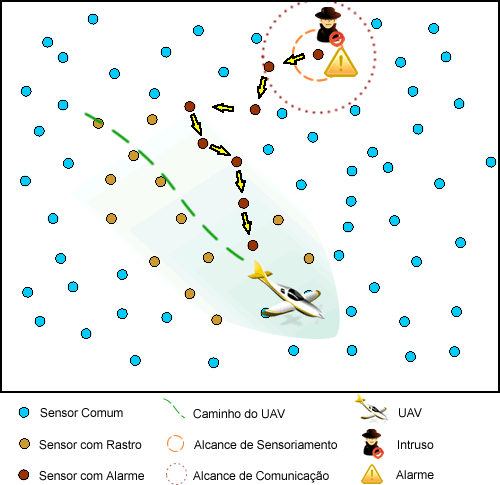
\includegraphics[width=12cm]{pictures/application.png}
 \caption{Propagação de um evento de interesse.}
  \label{fig:app}
 \end{figure}


\subsection{Reforço da Conectividade da Rede}
Esta seção aborda um último algoritmo deste trabalho. É válido salientar que este esta última técnica não influencia diretamente os resultados dos algoritmos apresentados anteriormente. Entretanto, as melhorias propostas nas seções anteriores propiciam o cenário para a implementação deste último algoritmo.

O algoritmo de Reforço de Conectividade da Rede utiliza os \vants que sobrevoam a área de interesse como nós sensores móveis, de modo que os \vants possam complementar a conectividade da rede em caso de falhas em nós sensores. Basicamente, falhas em nós sensores pode, ser consideradas como indisponibilidade de energia, falha em sensores, falha na interface de comunicação, etc.

Uma falha pode ser detectada pelo próprio nó, ou por seus vizinhos. Um exemplo de falha detectada pelo próprio nó é o mal funcionamento de um sensor, ou níveis muito baixos de energia. Falhas detectadas por vizinhos podem ser falência de um nó sensor ou ausência de interface de comunicação (não responde às mensagens de seus vizinhos), etc. A principal característica a se observar neste caso é que este problema pode ser mapeado em termos dos problemas anteriores; uma falha em um nó sensor pode ser considerada como um evento de interesse, e os rastros de feromônios podem ser utilizados para se carregar a mensagem de falha até o \vant mais próximo.

Ao receber uma mensagem de falha de um nó sensor, o \vant deve se preocupar em cobrir a conectividade da rede naquela região, atuando como um nó sensor da rede. Contudo, o \vant ainda possui suas responsabilidades em relação ao sistema de monitoramento de eventos. Para que se torne possível que o \vant realize todas as suas tarefas, a estratégia empregada é que o \vant apenas visite a área de falha em um determinado intervalo de tempo, e depois prossiga com seu itinerário.

Quando um \vant recebe mais de um alarme de falha de sensor, torna-se necessário que exista um escalonamento para que o \vant visite todas as regiões de falha. No desenvolvimento deste escalonamento, optou-se por uma implementação baseada em políticas. Neste caso, foi determinado um protocolo\footnote{Também pode ser considerado como uma Interface nos conceitos de Orientação a Objetos.} para a implementação de diferentes políticas. Isto permite que se desenvolva diferentes estratégias para o escalonamento das visitas às regiões de baixa cobertura da rede. Dentre estas políticas, podem ser destacadas:

\begin{description}
	\item[Agrupamento por Proximidade:] política para que o itinerário de visitas do \vant baseie-se em visitar sempre os nós mais próximos, de modo que a próxima região de visita seja a de menor distância do ponto atual.
	\item[Agrupamento Crítico:] é uma política em que se preocupa, principalmente, no agrupamento dos nós de acordo com a criticidade da região de falha. Nesta estratégia, a primeira região a ser visitada é a que possui mais avarias.
	\item[Agrupamento por Proximidade do \vant:] é uma especialização da primeira política. Todavia, mais complexa de se implementar, visto a necessidade de atualização da rota de acordo com a movimentação do \vant.
\end{description}

Uma característica interessante desta abordagem é a possibilidade de se alternar as políticas nos momentos mais adequados. Um \vant pode trabalhar com uma política A e ser reprogramado, ainda que em operação, para utilizar uma política B. Ainda mais, diversos \vants, no mesmo cenário, podem empregar diferentes políticas para o reforço de conectividade da rede. Ampliando, assim, o dinamismo do algoritmo abordado.

O protocolo para implementação desta políticas, apesar de dinâmico, apresenta-se simples, o desenvolvedor deve apenas oferecer um procedimento que compare duas regiões de falha.

Os blocos de código a seguir ilustram a implementação de uma política utilizada no trabalho.

\begin{lstlisting}[caption=Procolo (Interface) para implementação de Políticas de Agrupamento.]
package br.ufla.dcc.ucr.node.data;
public interface CoverageInfoComparator {
	int compare(CoverageInformation me, CoverageInformation other);
}
\end{lstlisting}


\begin{lstlisting}[caption=Implementação de Agrupamento Crítico.]
package br.ufla.dcc.ucr.node.data;
/**
*  Neste caso, coverage indica o grau de cobertura do no. Isto significa o quao danificado um no se encontra.
*/
public class SortByCoverage implements CoverageInfoComparator {
	@Override
	public int compare(CoverageInformation me, CoverageInformation other) {
		if (me.getCoverage() == other.getCoverage())
			return 0;
		if(me.getCoverage() < other.getCoverage()){
			return 1;
		}else{
			return -1;
		}
	}
}
\end{lstlisting}


\begin{lstlisting}[caption=Escolha da Política]
package br.ufla.dcc.ucr.node.data;
...
public class CoverageInformation implements Comparable<CoverageInformation> {
	//Escolha da politica de Agrupamento Critico. Basta mudar esta linha para trocar a politica.
	private CoverageInfoComparator compareStrategy = new SortByCoverage();
	...
	@Override
	public int compareTo(CoverageInformation other) {
		return this.compareStrategy.compare(this, other);
	}
	...
}
\end{lstlisting}

Para este trabalho, foram desenvolvidas as políticas de Agrupamento por Proximidade e de Agrupamento Crítico. Contudo, o modelo proposto permite que diversas extensões sejam feitas ao algoritmo.

O próximo capítulo demonstra os resultados dos experimentos realizados com os algoritmos apresentados neste capítulo.
